\documentclass[10pt, a4paper]{article}

\usepackage{ctex}
\usepackage{xeCJK}
\usepackage{caption}
\usepackage{geometry}
\geometry{
    left = 0.6in,
    right = 0.6in,
    top = 0.8in,
    bottom = 1.0in
}
\usepackage{amssymb}
\usepackage{amsbsy}
\usepackage{amsmath}
\usepackage{xcolor}
\usepackage{mathrsfs}
\usepackage{graphicx}
\usepackage{tasks}
\settasks{
    label = \Alph*. ,
    label-width = 16pt
}

\newcommand{\Title}[3]{
    \begin{center}
        \Large \textbf{中国电子学会 #1~年~#2~月 Scratch~#3级考试}
    \end{center}
}
\newcommand{\TimeAndName}[1]{
    \begin{center}
        考试时间:~#1~ 分钟 \qquad\qquad\qquad\qquad 姓名:\underline{\quad\quad\quad\quad}
    \end{center}
}
\pagestyle{empty}
\begin{document}
    \Title{2021}{9}{一}
    
    \TimeAndName{60}
    
    {\noindent\heiti 第一部分、单选题(共 25 题,每题 2 分,共50分.)}

    \begin{enumerate}
        % 1
        \item  如下图所示,小明想要做一个文字逐字出现的动画效果,他画出了程序的流程图,以下哪个程序可以实现?(\qquad)
        \begin{figure}[htbp]
            \centering
            \begin{minipage}{.28\textwidth}
                \centering
                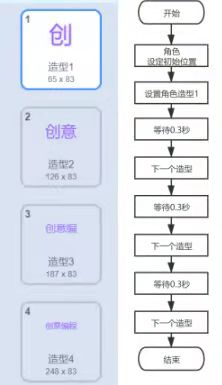
\includegraphics[width=.6\textwidth]{1.jpg}
            \end{minipage}
            \begin{minipage}{.68\textwidth}
                \centering
                \begin{tasks}(4)
                    \task 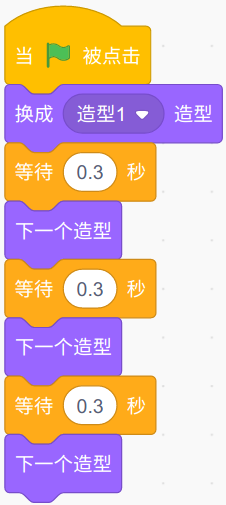
\includegraphics[width=.17\textwidth]{1a.png}
                    \task 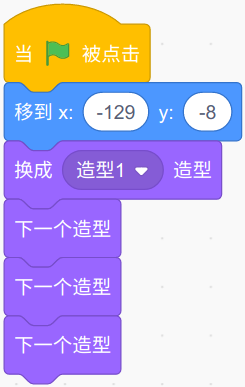
\includegraphics[width=.17\textwidth]{1b.png}
                    \task 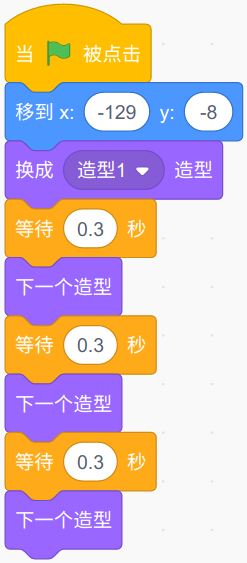
\includegraphics[width=.17\textwidth]{1c.png}
                    \task 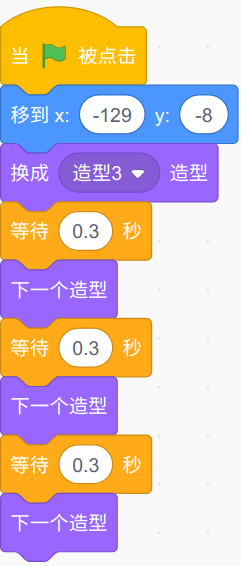
\includegraphics[width=.15\textwidth]{1d.png}
                \end{tasks}
            \end{minipage}
        \end{figure}

        % 2
        \item 如下图所示,分别是2层和3层三角形金字塔,请问如果是6层三角形金字塔由几个小三角形组成?(\qquad)
        \begin{tasks}(4)
            \task 24
            \task 30
            \task 36
            \task 42
        \end{tasks}

        % 3
        \item 下面哪一项是“控制”模块中的积木?(\qquad)
        \begin{tasks}(4)
            \task 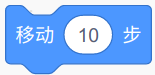
\includegraphics[width=.1\textwidth]{3a.png}
            \task 
\includegraphics[width=.1\textwidth]{3b.png}
            \task 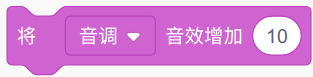
\includegraphics[width=.18\textwidth]{3c.png}
            \task 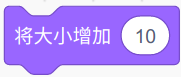
\includegraphics[width=.12\textwidth]{3d.png}
        \end{tasks}

        \begin{figure}[htbp]
            \centering
            \begin{minipage}[t]{.2\textwidth}
                \centering
                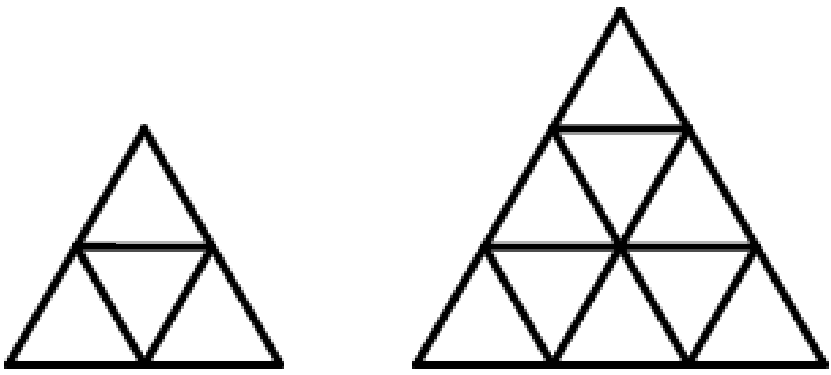
\includegraphics[width=1\textwidth]{2.png}
                \caption*{第2题}
            \end{minipage}
            \begin{minipage}[t]{.35\textwidth}
                \centering
                \begin{minipage}[t]{.18\textwidth}
                    \centering
                    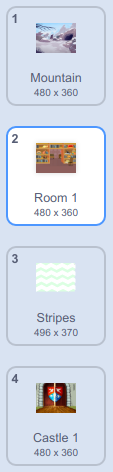
\includegraphics[width=.7\textwidth]{6-1.png}
                \end{minipage}
                \begin{minipage}[t]{.68\textwidth}
                    \centering
                    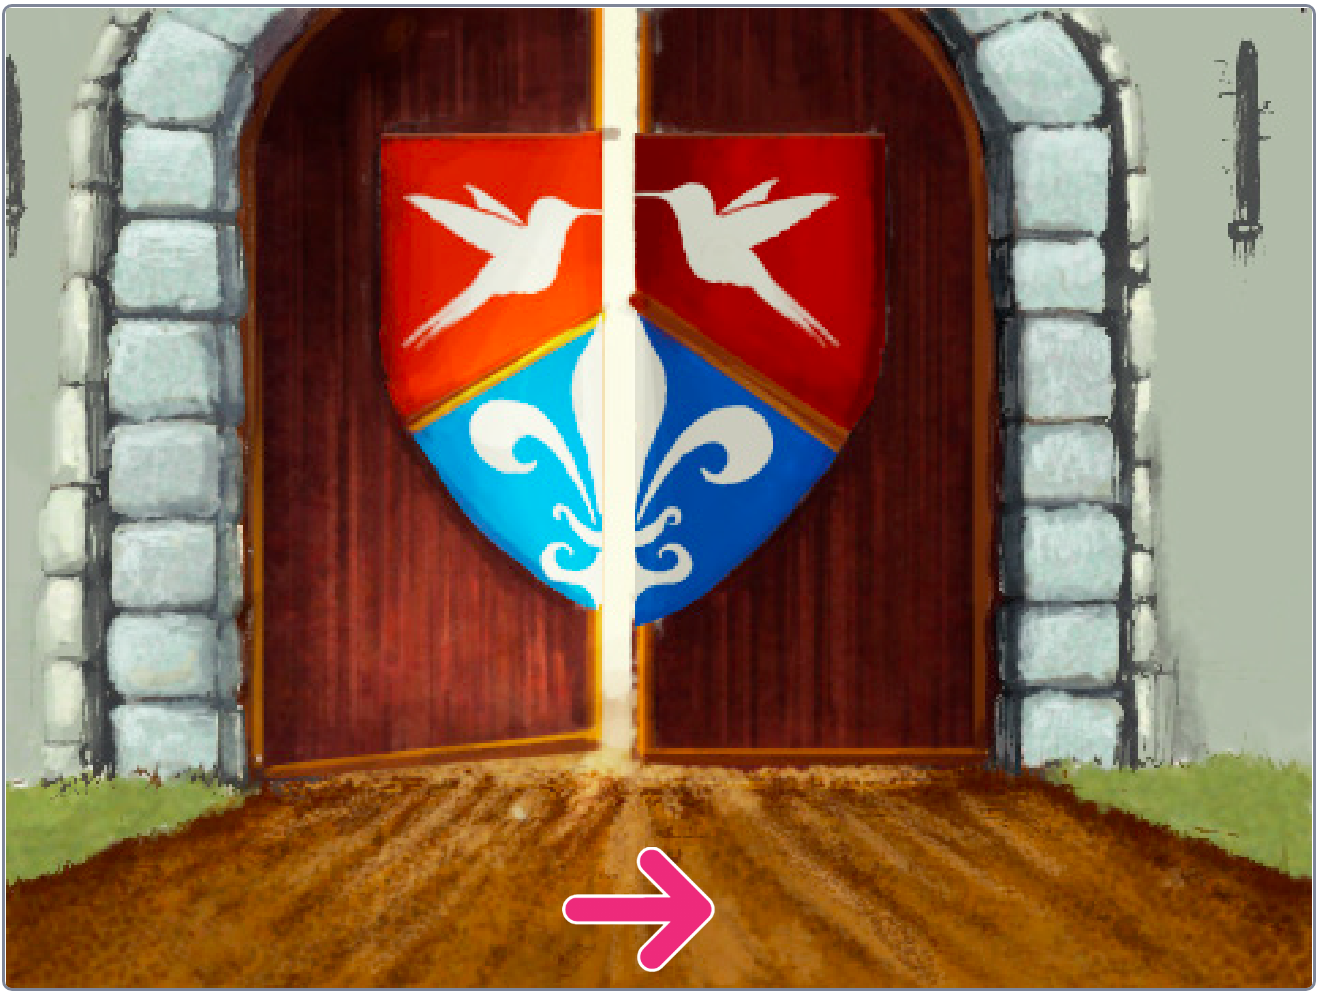
\includegraphics[width=\textwidth]{6-2.png}
                \end{minipage}
                \caption*{第6题}
            \end{minipage}
            \begin{minipage}[t]{.35\textwidth}
                \centering
                \begin{minipage}[t]{.18\textwidth}
                    \centering
                    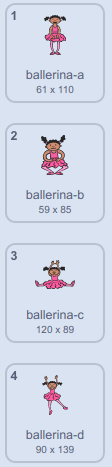
\includegraphics[width=.7\textwidth]{7-1.png}
                \end{minipage}
                \begin{minipage}[t]{.68\textwidth}
                    \centering
                    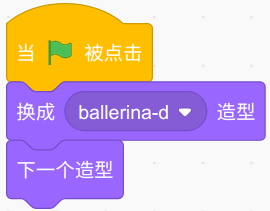
\includegraphics[width=\textwidth]{7-2.png}
                \end{minipage}
                \caption*{第7题}
            \end{minipage}
        \end{figure}

        % 4
        \item 下面哪种不是角色旋转方式?(\qquad)
        \begin{tasks}(4)
            \task 左右翻转
            \task 上下翻转
            \task 不可旋转
            \task 任意旋转
        \end{tasks}

        % 5
        \item 下面哪个区域用来编写程序?(\qquad)
        \begin{tasks}(4)
            \task 脚本区
            \task 角色区
            \task 舞台区
            \task 模块区
        \end{tasks}

        % 6
        \item 小明想要做一个如上图所示的简易电子相册,点击图中“方向箭头”,就切换到下一个舞台背景,以下能实现该功能的是?(\qquad)
        \begin{tasks}(4)
            \task 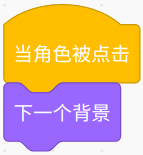
\includegraphics[width=.07\textwidth]{6a.png}
            \task 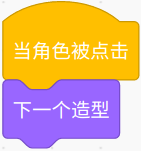
\includegraphics[width=.07\textwidth]{6b.png}
            \task 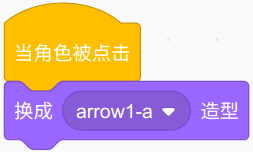
\includegraphics[width=.13\textwidth]{6c.png}
            \task 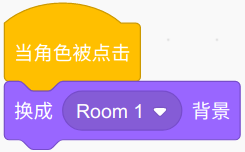
\includegraphics[width=.13\textwidth]{6d.png}
        \end{tasks}
        
        % 7
        \item Ballerina是个喜欢跳舞的女孩,她有4个造型,执行完下图的程序后,Ballerina换成了第几个造型?(\qquad)
        \begin{tasks}(4)
            \task 1
            \task 2
            \task 3
            \task 4
        \end{tasks}
           
        \newpage
        % 8
        \item 如下图所示,Batter角色有几个造型?(\qquad)
        \begin{tasks}(4)
            \task 1
            \task 2
            \task 3
            \task 4
        \end{tasks}

        % 9
        \item 如果小猫想在舞台上展示多种时尚的穿戴,应该使用以下哪个积木?(\qquad)
        \begin{tasks}(4)
            \task 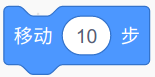
\includegraphics[width=.1\textwidth]{9a.png}
            \task 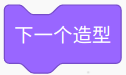
\includegraphics[width=.08\textwidth]{9b.png}
            \task 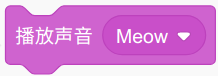
\includegraphics[width=.13\textwidth]{9c.png}
            \task 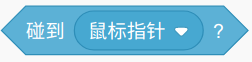
\includegraphics[width=.15\textwidth]{9d.png}
        \end{tasks}

        \begin{figure}[htbp]
            \centering
            \begin{minipage}[t]{.3\textwidth}
                \centering
                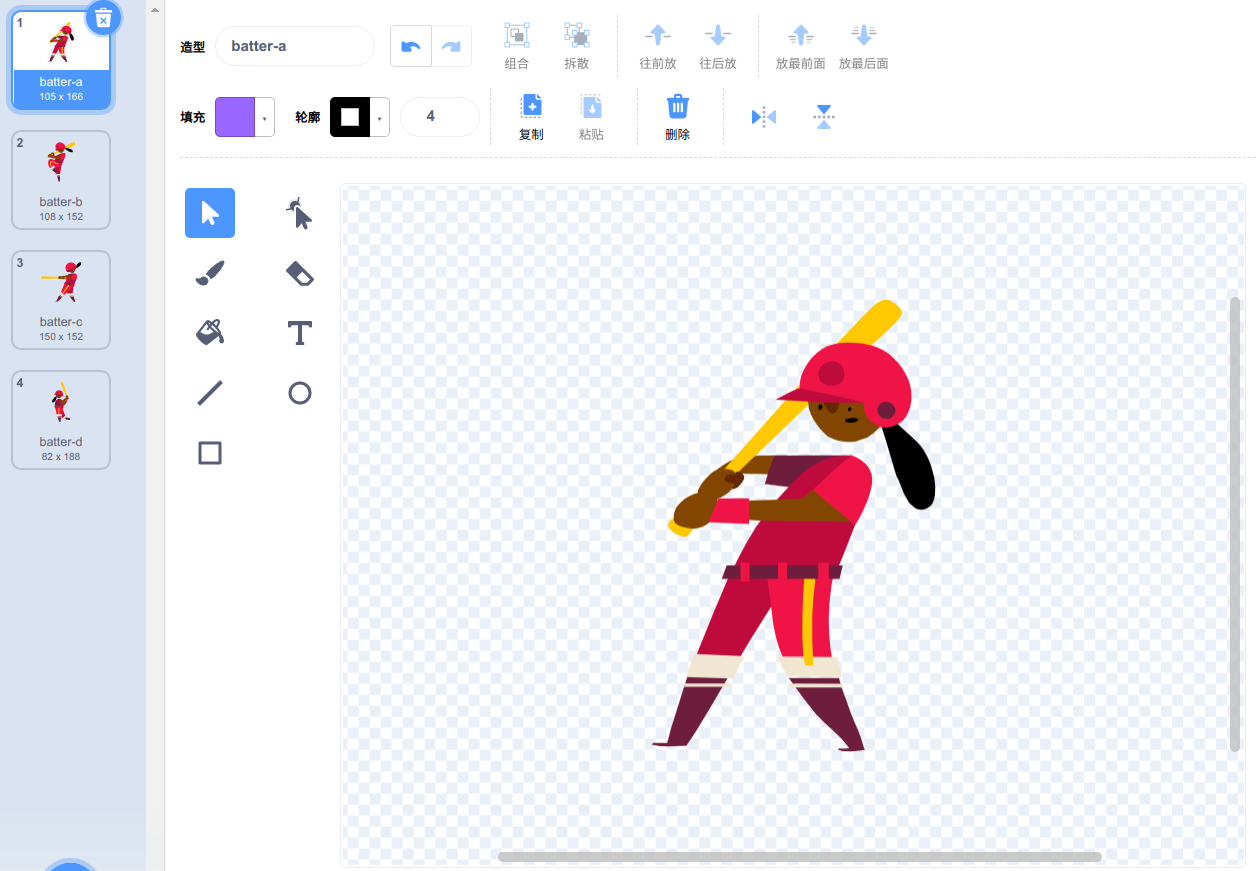
\includegraphics[width=\textwidth]{8.png}
                \caption*{第8题}
            \end{minipage}
            \begin{minipage}[t]{.1\textwidth}
                \centering
                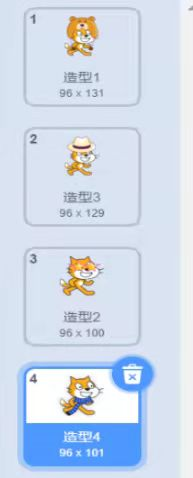
\includegraphics[width=0.85\textwidth]{9.jpg}
                \caption*{第9题}
            \end{minipage}
            \begin{minipage}[t]{.28\textwidth}
                \centering
                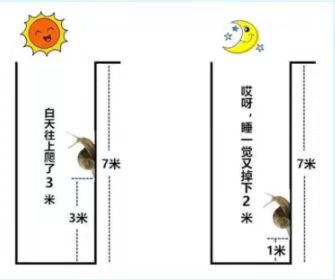
\includegraphics[width=0.9\textwidth]{10.jpg}
                \caption*{第10题}
            \end{minipage}
            \begin{minipage}[t]{.28\textwidth}
                \centering
                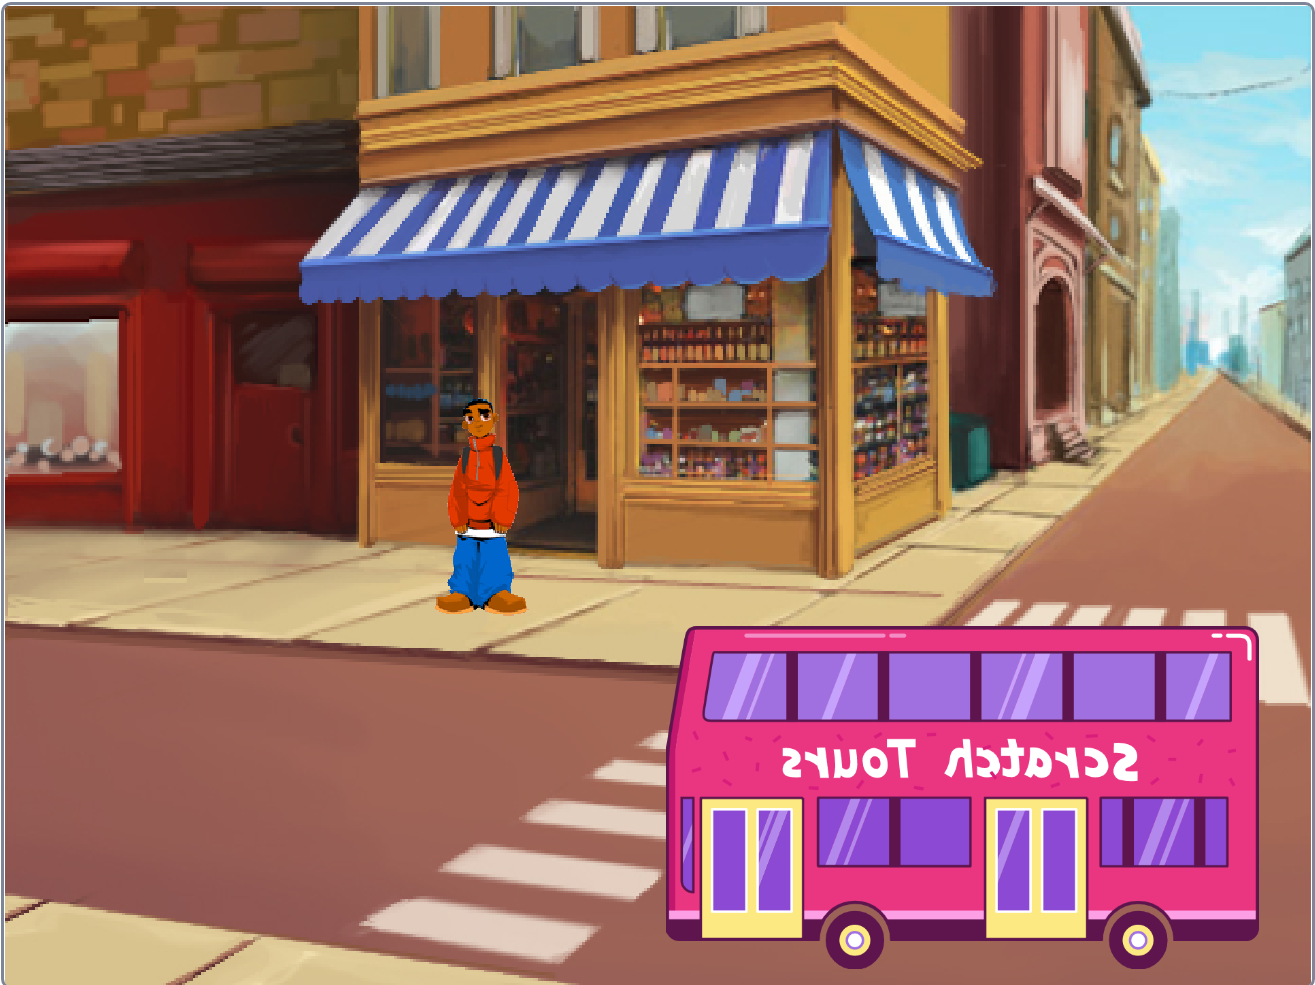
\includegraphics[width=\textwidth]{14.png}
                \caption*{第14题}
            \end{minipage}
        \end{figure}

        % 10
        \item 如上图所示,井深7米,蜗牛从井底往上爬,白天爬3米,晚上往下掉2米,问蜗牛几天能从井里爬出来?(\qquad)
        \begin{tasks}(4)
            \task 4
            \task 5
            \task 6
            \task 7
        \end{tasks}

        % 11
        \item 小明想在Scratch中导入一段自己在网上下载的音乐作为背景音乐,应该使用哪个按钮?(\qquad)
        \begin{tasks}(4)
            \task 
\includegraphics[width=.03\textwidth]{11a.png}
            \task 
\includegraphics[width=.03\textwidth]{11b.png}
            \task 
\includegraphics[width=.03\textwidth]{11c.png}
            \task 
\includegraphics[width=.03\textwidth]{11d.png}
        \end{tasks}
        
        % 12
        \item  小猫过生日,我们为它播放生日快乐歌,播放完毕后,小猫高兴的“喵”了一声,下面哪个程序可以实现这个场景?(\qquad)
        \begin{tasks}(4)
            \task 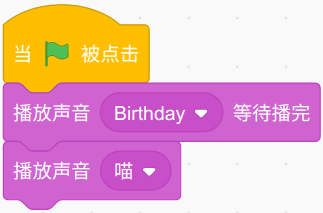
\includegraphics[width=.15\textwidth]{12a.png}
            \task 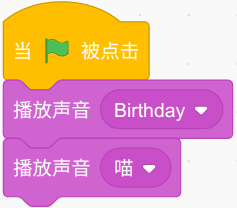
\includegraphics[width=.12\textwidth]{12b.png}
            \task 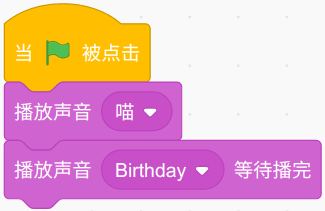
\includegraphics[width=.17\textwidth]{12c.png}
            \task 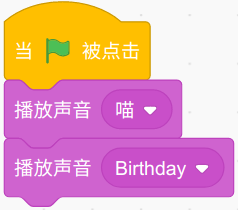
\includegraphics[width=.12\textwidth]{12d.png}
        \end{tasks}

        % 13
        \item 看图找规律,图中
\includegraphics[width=.2\textwidth]{13.jpg}红框中的图形应该是?(\qquad)
        \begin{tasks}(4)
            \task 
\includegraphics[width=.03\textwidth]{13a.jpg}
            \task 
\includegraphics[width=.03\textwidth]{13b.jpg}
            \task 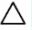
\includegraphics[width=.03\textwidth]{13c.jpg}
            \task 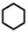
\includegraphics[width=.03\textwidth]{13d.jpg}
        \end{tasks}

        % 14
        \item 小明觉得巴士的声音太吵了,下面哪个选项可以把音量调小为原来的一半?(\qquad)
        \begin{tasks}(2)
            \task 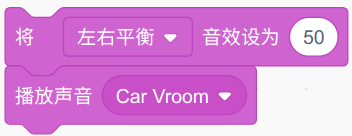
\includegraphics[width=.25\textwidth]{14a.png}
            \task 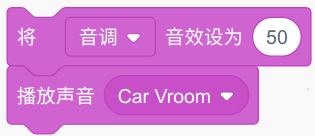
\includegraphics[width=.25\textwidth]{14b.png}
            \task 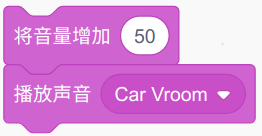
\includegraphics[width=.18\textwidth]{14c.png}
            \task 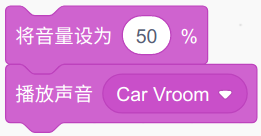
\includegraphics[width=.18\textwidth]{14d.png}
        \end{tasks}
    
        \newpage
        % 15
        \item 角色“Apple”在舞台中央,面向90度,下图为默认角色“Apple”的程序,运行后,角色在舞台的?(\qquad)
        \begin{tasks}(4)
            \task 左上角
            \task 左下角
            \task 右上角
            \task 右下角
        \end{tasks}

        % 16
        \item 默认的小猫角色在面向左的时候头朝下,请问使用下面哪个积木可以让小猫面向左的时候头朝上?(\qquad)
        \begin{tasks}(4)
            \task 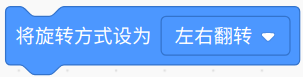
\includegraphics[width=.18\textwidth]{16a.png}
            \task 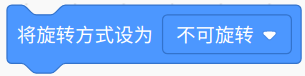
\includegraphics[width=.18\textwidth]{16b.png}
            \task 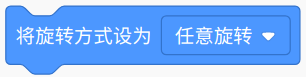
\includegraphics[width=.18\textwidth]{16c.png}
            \task 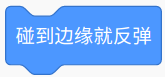
\includegraphics[width=.1\textwidth]{16d.png}
        \end{tasks}

        % 17
        \item 编程让小猫右转15度,小猫是围绕下面哪个选项旋转的?(\qquad)
        \begin{tasks}(4)
            \task 角色最下方
            \task 角色最右方
            \task 角色中心点
            \task 角色中间
        \end{tasks}

        % 18
        \item 下面说法不正确的是?(\qquad)
        \begin{tasks}(2)
            \task 可以通过麦克风录音
            \task 可以通过导入方式从已有的文件中导入声音
            \task 可以一次性导入声音库中的多个声音
            \task 可以随机导入声音库中的声音
        \end{tasks}

        \begin{figure}[htbp]
            \centering
            \begin{minipage}[t]{.15\textwidth}
                \centering
                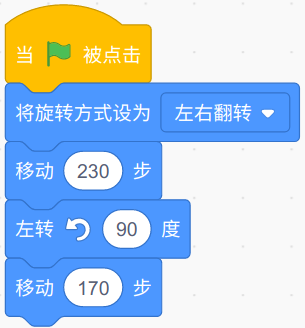
\includegraphics[width=\textwidth]{15.png}
                \caption*{第15题}
            \end{minipage}
            \begin{minipage}[t]{.22\textwidth}
                \centering
                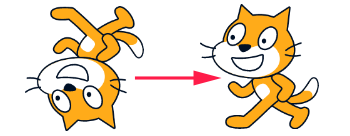
\includegraphics[width=\textwidth]{16.png}
                \caption*{第16题}
            \end{minipage}
            \begin{minipage}[t]{.1\textwidth}
                \centering
                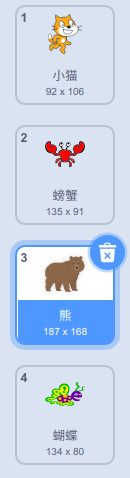
\includegraphics[width=0.7\textwidth]{21.png}
                \caption*{第21题}
            \end{minipage}
        \end{figure}

        % 19
        \item  一阵微风吹过,下图中的风车旋转了半圈180度,下面哪个程序能实现这个功能?(\qquad)
        \begin{figure}[htbp]
            \centering
            \begin{minipage}{.28\textwidth}
                \centering
                \includegraphics[width=\textwidth]{19.jpg}
                \caption*{第19题}
            \end{minipage}
            \begin{minipage}{.68\textwidth}
                \centering
                \begin{tasks}(4)
                    \task \includegraphics[width=.1\textwidth]{19a.png}
                    \task \includegraphics[width=.12\textwidth]{19b.png}
                    \task \includegraphics[width=.12\textwidth]{19c.png}
                    \task \includegraphics[width=.15\textwidth]{19d.png}
                \end{tasks}
            \end{minipage}
        \end{figure}

        % 20
        \item 每次完成一个Scratch作品,为了以后继续使用或者编辑,要求我们务必完成哪项操作?(\qquad)
        \begin{tasks}(4)
            \task 删除文件
            \task 保存文件
            \task 新建文件
            \task 复制文件
        \end{tasks}

        % 21
        \item 如上图所示,角色有四个动物造型,当前造型为熊,下列哪个程序执行完后,造型不能切换成螃蟹?(\qquad)
        \begin{tasks}(4)
            \task \includegraphics[width=.15\textwidth]{21a.png}
            \task \includegraphics[width=.12\textwidth]{21b.png}
            \task \includegraphics[width=.06\textwidth]{21c.png}
            \task \includegraphics[width=.15\textwidth]{21d.png}
        \end{tasks}

        \newpage
        % 22
        \item 如下图所示,下面哪个选项的程序可以实现人物从起点走到终点?(\qquad)
        \begin{tasks}(4)
            \task \includegraphics[width=.1\textwidth]{22a.png}
            \task \includegraphics[width=.1\textwidth]{22b.png}
            \task \includegraphics[width=.1\textwidth]{22c.png}
            \task \includegraphics[width=.1\textwidth]{22d.png}
        \end{tasks}

        \begin{figure}[htbp]
            \centering
            \begin{minipage}[t]{.3\textwidth}
                \centering
                \includegraphics[width=\textwidth]{22.jpg}
                \caption*{第22题}
            \end{minipage}
            \begin{minipage}[t]{.25\textwidth}
                \centering
                \includegraphics[width=\textwidth]{23.jpg}
                \caption*{第23题}
            \end{minipage}
            \begin{minipage}[t]{.28\textwidth}
                \centering
                \begin{minipage}[t]{.6\textwidth}
                    \centering
                    \includegraphics[width=\textwidth]{25-1.png}
                \end{minipage}
                \begin{minipage}[t]{.28\textwidth}
                    \centering
                    \includegraphics[width=\textwidth]{25-2.png}
                \end{minipage}
                \caption*{第25题}
            \end{minipage}
        \end{figure}

        % 23
        \item 如上图所示,下面哪个选项可以把从网上下载的卡通素材导入到Scratch中作为角色使用?(\qquad)
        \begin{tasks}(2)
            \task 从本地文件夹中上传角色
            \task 从角色库中选择
            \task 直接复制粘贴角色到Scratch中
            \task 绘制新角色
        \end{tasks}

        % 24
        \item 小明去食堂排队打饭,他前面有2人,后面有3人,那小明排在第几位?(\qquad)
        \begin{tasks}(4)
            \task 2
            \task 3
            \task 4
            \task 5
        \end{tasks}
        
        % 25
        \item 新年音乐会上,小猫准备进行踩球表演,舞台、角色以及角色造型如上图所示,下面说法正确的是?(\qquad)
        \begin{tasks}
            \task 舞台使用音乐会背景,造型只需要一只小猫
            \task 舞台使用音乐会背景,造型由小猫踩球的不同动作组成
            \task 角色使用音乐会背景,造型由小猫踩球的不同动作组成
            \task 角色是音乐会背景,造型只需要一只小猫
        \end{tasks}
    \end{enumerate}

    \newpage
    {\noindent\heiti 第二部分、判断题(共 10 题,每题 2 分,共20分.)}
    \begin{enumerate}
        \setcounter{enumi}{25}
        % 26
        \item 下图中每个水果表示一个数,那么桃子表示3、香蕉表示6、梨表示4.(\qquad)
        
        \begin{figure}[h!]
            \centering
            \begin{minipage}[t]{.18\textwidth}
                \centering
                \includegraphics[width=\textwidth]{26.jpg}
                \caption*{第26题}
            \end{minipage}
            \begin{minipage}[t]{.18\textwidth}
                \centering
                \includegraphics[width=\textwidth]{33.png}
                \caption*{第33题}
            \end{minipage}
        \end{figure}

        %27
        \item 位图在放大一定倍数后边缘会出现锯齿,而矢量图不会.(\qquad)
        
        %28
        \item 角色的旋转模式,对于角色的旋转效果没有任何影响.(\qquad)
  
        %29
        \item Scratch支持的声音格式有两种:“wav”和“mp3”格式.(\qquad)
        
        %30
        \item 程序有多个小猫角色,我们可以在角色列表区更改角色的名称,这样能更好区分角色.(\qquad)
        
        %31
        \item “播放声音等待完毕”和“播放声音”两个积木使用效果是一样的.(\qquad)
        
        %32
        \item Scratch中,一个舞台上最多只可以添加一个角色.(\qquad)
        
        %33
        \item 可以把角色包括它的程序一起导出,在另外一个程序中使用下面按钮导入.(\qquad)
        
        %34
        \item 不小心连续删除了舞台上的3个角色,使用“编辑”里的“恢复”功能就可以重新恢复这3个角色.(\qquad)
        
        %35
        \item 无论是角色的造型编号,还是舞台的背景编号都是从1开始.(\qquad)
    \end{enumerate}

    {\noindent\heiti 第三部分、编程题(共 2 题,共30分.)}
    \begin{enumerate}
        \setcounter{enumi}{35}
        
        % 36
        \item 无奈的Jaime:
        
        1. 准备工作
        \begin{tasks}[label = (\arabic*)]
            \task 添加背景:Bedroom3;
            \task 删除默认小猫角色,添加角色:Jaime;
            \task 给Jaime角色添加声音:Laugh1、Scream1.
        \end{tasks}
        2. 功能实现
        \begin{tasks}[label = (\arabic*)]
            \task 点击绿旗,Jaime出现在舞台左下角,面向右,造型为jaime walking-a;
            \task 依次播放完2中声音Laugh1和声音Scream1;
            \task 当播放完所有声音后,Jaime从舞台左侧走到右侧,再从右侧走到左侧,边走边思考“怎么办?”;(注意走的过程中脚不能朝上,并且朝哪个方向走Jaime就面朝哪边)
            \task 走完后,切换成造型jaime-a,然后说“sorry!”2秒.
        \end{tasks}
        \begin{center}
            \includegraphics[width=.3\textwidth]{36.png}
        \end{center}

        %37
        \item 小狗进圈:
        
        1. 准备工作
        \begin{tasks}[label = (\arabic*)]
            \task 背景:根据右图绘制背景;
            \task 删除小猫角色,添加角色:“Dog2”;
            \task 给Dog2添加声音:Dog2.
        \end{tasks}
        2. 功能实现
        \begin{tasks}[label = (\arabic*)]
            \task 舞台颜色为蓝色,绘制3个椭圆,椭圆的大小要能容下小狗,内部填充白色,椭圆的间距尽量相等;
            \task 点击绿旗,程序开始,Dog2位于最左侧椭圆内,面向右侧,造型为“dog2-a”;
            \task 按下空格键,Dog2发出“Dog2”叫声、切换下一个造型,向右跳到下一个椭圆.
            
            \textcolor{orange}{注意:点击绿旗后,只测试两次按下空格键即可,第一次按一下能跳到第二个椭圆,第二次按下能跳到第三个椭圆.}
        \end{tasks}
        \begin{center}
            \includegraphics[width=.3\textwidth]{37.png}
        \end{center}
    \end{enumerate}
\end{document}